\documentclass[UTF8,a4paper,zihao=-4,fontset=fandol]{ctexart}

\usepackage[left=2.5cm,right=2.5cm,top=2.5cm,bottom=2.5cm]{geometry}
\usepackage{setspace}
\usepackage{amsmath,amssymb,amsthm,mathtools,bm}
\usepackage{graphicx}
\usepackage{booktabs,tabularx,array,longtable,multirow}
\usepackage{caption}
\usepackage{float}
\usepackage{enumitem}
\usepackage{fancyhdr}
\usepackage{hyperref}
\usepackage{xcolor}
\usepackage{microtype}
\usepackage{needspace}
\usepackage{etoolbox}
\usepackage{lastpage}
\usepackage{seqsplit}

\hypersetup{hidelinks,pdfauthor={邢若琦},pdftitle={SPN型置换相关矩阵坐标的可认证稀疏路线壳求和}}

% 字体与版式
% 不提交字体文件; 英文字体按系统可用性回退, 中文模板字体使用 TeX Live 自带 Fandol.
\IfFontExistsTF{Times New Roman}
  {\setmainfont{Times New Roman}}
  {\IfFontExistsTF{TeX Gyre Termes}{\setmainfont{TeX Gyre Termes}}{}}
\setCJKmainfont[BoldFont=FandolSong-Bold.otf,ItalicFont=FandolKai-Regular.otf]{FandolSong-Regular.otf}
\setCJKsansfont[BoldFont=FandolHei-Bold.otf]{FandolHei-Regular.otf}
\setCJKmonofont{FandolFang-Regular.otf}
\setCJKfamilyfont{fang}{FandolFang-Regular.otf}
\newcommand{\fangsongcustom}{\CJKfamily{fang}}
\setlength{\parindent}{2em}
\setlength{\parskip}{0pt}
\onehalfspacing
\punctstyle{plain}
\setlength{\emergencystretch}{2em}

% 标题层级: 一级中文序号, 二级数字序号, 三级 1.1
\ctexset{
  section={
    name={,、},
    number=\chinese{section},
    format=\heiti\zihao{3},
    beforeskip=1.2em,
    afterskip=0.6em,
    indent=0pt,
    aftername=\hspace{0pt}
  },
  subsection={
    name={,},
    number=\arabic{subsection}.,
    format=\heiti\zihao{-3},
    beforeskip=0.9em,
    afterskip=0.4em,
    indent=2em,
    aftername=\hspace{0.5em}
  },
  subsubsection={
    name={,},
    number=\arabic{subsection}.\arabic{subsubsection},
    format=\heiti\zihao{-3},
    beforeskip=0.7em,
    afterskip=0.3em,
    indent=2em,
    aftername=\hspace{0.5em}
  }
}

% 公式编号: (x.y), x 为一级标题阿拉伯序号
\numberwithin{equation}{section}
\renewcommand{\theequation}{\arabic{section}.\arabic{equation}}

% 图表与页码
\renewcommand{\figurename}{图}
\renewcommand{\tablename}{表}
\DeclareCaptionFont{captionsong}{\songti\zihao{5}}
\DeclareCaptionFont{captionhei}{\heiti\zihao{5}}
\captionsetup{font=captionsong,labelfont=captionhei,labelsep=quad,justification=centering,singlelinecheck=false}
\captionsetup[table]{position=top,skip=4pt}
\captionsetup[figure]{position=bottom,skip=6pt}
\setlength{\textfloatsep}{10pt plus 2pt minus 2pt}
\setlength{\floatsep}{8pt plus 2pt minus 2pt}
\setlength{\intextsep}{8pt plus 2pt minus 2pt}

\pagestyle{fancy}
\fancyhf{}
\renewcommand{\headrulewidth}{0pt}
\fancyfoot[C]{\zihao{5}\thepage}

% 定理环境
\theoremstyle{definition}
\newtheorem{definition}{定义}
\theoremstyle{plain}
\newtheorem{theorem}{定理}
\newtheorem{proposition}[theorem]{命题}
\theoremstyle{remark}
\newtheorem*{remark}{说明}

% 表格
\newcolumntype{Y}{>{\centering\arraybackslash}X}
\newcolumntype{L}{>{\raggedright\arraybackslash}X}
\newcolumntype{C}[1]{>{\centering\arraybackslash}p{#1}}
\renewcommand{\arraystretch}{1.25}

% 常用数学符号: 矩阵使用粗斜体, 路线使用花体
\newcommand{\MatM}{\bm{M}}
\newcommand{\MatR}{\bm{R}}
\newcommand{\MatL}{\bm{L}}
\newcommand{\Route}{\mathcal{R}}
\newcommand{\Hull}{\mathcal{H}}
\newcommand{\supp}{\operatorname{supp}}
\newcommand{\cor}{\operatorname{cor}}
\newcommand{\wt}{\operatorname{wt}_{\mathrm{nib}}}
\newcommand{\score}{\operatorname{score}}
\newcommand{\code}[1]{\texttt{#1}}

\begin{document}
\zihao{4}

% 标题页(同时为摘要首页)
\begin{center}
  {\heiti\zihao{-2} SPN 型置换相关矩阵坐标的可认证稀疏路线壳求和\par}
  \vspace{0.45em}
  {\heiti\zihao{3} ——路线壳引导的稀疏动态规划在矩阵连乘元素逼近中的应用\par}
  \vspace{1.1em}
  {\fangsongcustom\zihao{4} 邢若琦\quad 刘振华(指导老师)\par}
  \vspace{0.35em}
  {\songti\zihao{-4} 西安电子科技大学\quad 18957444596@163.com\par}
  \vspace{0.25em}
  {\songti\zihao{-4} 战队名称: 稳稳接住\quad 战队序号: 0000002243\quad 西北赛区\par}
\end{center}
\vspace{0.9em}

\noindent{\songti\zihao{4}\bfseries 摘要: }
{\songti\zihao{4}
本文研究由分组密码轮函数相关矩阵诱导的结构化坐标计算问题. 给定轮数 $r$、输入掩码 $u$ 与输出掩码 $v$, 目标是计算由 $3r$ 个 $2^{32}\times 2^{32}$ 相关矩阵连乘得到的坐标 $\bm{M}(r)[v,u]$. 直接精确路径需枚举 $2^{32}$ 个明文, 难以支撑大规模候选发现. 本文提出可认证稀疏路线壳求和: 利用八个并联 S 盒相关矩阵的克罗内克积结构枚举非零局部分支, 利用行移位与列混合层的转置传播关系确定唯一后继掩码, 并对到达同一掩码的路线贡献进行带符号聚合. 候选阶段允许截断以发现高价值端点; 最终结果仅保留局部分支、S 层元组和聚合状态均未截断的运行. 本文证明, 对固定 $(r,u)$, 该完整性证书蕴含 $A_r=\bm{R}^{r}e_u$, 从而任意输出端点满足 $A_r[v]=\bm{M}(r)[v,u]$. 在评测实例上, 最终结果集包含 138338 条有效记录, 总分为 105843.622442471292742994; 全部记录通过无截断审计, 复现不匹配数为 0. 18 条方式一独立精确抽样复核全部一致, 其中包括 4 条 $r=3$ 活跃二字补充样本. 结果表明, 本文方法能够在不枚举明文空间的前提下, 对低活跃掩码区域中的完整线性壳进行可证明、可审计的稀疏求和. }

\vspace{0.6em}
\noindent{\songti\zihao{4}\bfseries 关键词: }{\songti\zihao{4} 相关矩阵; 线性壳; 稀疏动态规划; 线性密码分析; 矩阵连乘}

\section{引言}

线性密码分析以输入掩码与输出掩码之间的相关度刻画密码变换对线性关系的偏离\textsuperscript{[3--5]}. 对多轮替换-置换网络(substitution-permutation network, SPN)而言, 轮函数复合对应相关矩阵的乘积, 而指定输入、输出掩码之间的相关度就是该乘积矩阵的一个坐标. 第十一届全国高校密码数学挑战赛赛题三给出了一个 32 比特 SPN 型置换、矩阵坐标 $\bm{M}(r)[v,u]$、方式一与方式二、计分规则以及提交格式\textsuperscript{[1]}; 官方示例程序以 $2^{32}$ 个明文枚举计算相关度, 构成独立精确基准\textsuperscript{[2]}.

本文考虑如下抽象问题: 给定由并联 S 盒层和可逆线性层交替组成的 SPN 型置换, 计算其 $r$ 轮相关矩阵中的指定坐标 $\bm{M}(r)[v,u]$. 困难不在单个相关矩阵元素的定义, 而在多轮复合后线性路线数量快速增长. 本文的目标是在不枚举明文空间的前提下, 利用 S 盒层局部性与线性层确定性传播, 对低活跃掩码区域中的完整线性壳进行可认证稀疏求和.

一轮结构由 S 盒层 $SC$、行移位层 $SR$ 和列混合层 $MC$ 构成. S 盒层相关矩阵是八个 4 比特局部相关矩阵的克罗内克积; $SR$ 与 $MC$ 是可逆线性层, 其相关矩阵的非零位置由转置掩码关系决定. 因此, 目标坐标可以在掩码路线空间中展开为线性壳和, 而不必逐点枚举明文. 本文方法并非追踪单条最大路线, 而是维护从固定输入掩码到各中间掩码的带符号路线贡献和. 候选阶段可以采用截断式搜索; 最终数值生成只接受通过无截断认证的运行.

本文主要贡献如下:
\begin{enumerate}[label=\arabic*.,leftmargin=2.8em,itemsep=0.2em]
  \item 建立相关矩阵坐标、组件级线性路线和完整线性壳之间的统一模型, 明确一轮矩阵与路线符号的区别: $\bm{R}$ 始终表示一轮相关矩阵, $\Route$ 始终表示一条线性路线.
  \item 提出可认证稀疏路线壳求和, 通过 S 盒非零分支、线性层唯一传播和端点带符号聚合, 在掩码路线空间中计算目标坐标.
  \item 给出无截断认证的数学定义与归纳证明, 证明固定 $(r,u)$ 的认证运行满足 $A_r=\bm{R}^r e_u$.
  \item 给出按唯一 $(r,u)$ 计量的结构复杂度分析, 并以全量审计、精确抽样复核和结果重建构成可复核证据链.
\end{enumerate}

\begin{table}[H]
\centering
\caption{方法谱系对比}
\label{tab:method-spectrum}
\zihao{-4}
\begin{tabularx}{\textwidth}{C{2.8cm}L C{1.7cm} C{1.9cm} C{2.1cm} L}
\toprule
方法 & 计算对象 & 枚举明文 & 聚合路线壳 & 完整性证书 & 主要用途 \\
\midrule
方式一明文枚举 & $\cor_{HS(r)}(v,u)$ & 是 & 隐式 & 是 & 独立精确验证基准 \\
单路线近似 & 最大单条路线贡献 & 否 & 否 & 否 & 启发式候选搜索 \\
截断式路线壳搜索 & 部分路线壳和 & 否 & 是 & 否 & 候选发现 \\
本文可认证完整路线壳求和 & 完整线性壳和 & 否 & 是 & 是 & 最终数值生成与正确性声明 \\
\bottomrule
\end{tabularx}
\end{table}

截断式路线壳搜索与最终可认证求和共享同一状态转移, 但承担不同功能: 前者只用于候选发现, 后者用于最终数值生成和正确性声明.

\section{符号与问题建模}

\subsection{掩码空间与坐标约定}

所有输入与输出掩码均属于 $\mathcal X=\mathbb F_2^{32}$, 并视为八个 4 比特字的拼接:
\begin{equation}
\mathcal X=(\mathbb F_2^4)^8.
\label{eq:mask-space}
\end{equation}
32 比特十六进制掩码 $\mathtt{0x}x_0x_1\cdots x_7$ 对应向量 $(x_0,x_1,\ldots,x_7)$, 其中 $x_0$ 为最高 4 比特, $x_7$ 为最低 4 比特. 本文使用 $\bm{M}[v,u]$ 表示矩阵第 $v$ 行、第 $u$ 列元素, 其中 $u$ 为输入掩码, $v$ 为输出掩码.

\subsection{归一化相关矩阵}

对函数 $F:\mathbb F_2^n\to\mathbb F_2^n$, 归一化线性相关度定义为
\begin{equation}
\cor_F(v,u)=2^{-n}\sum_{x\in\mathbb F_2^n}(-1)^{u^\top x\oplus v^\top F(x)}.
\label{eq:corr-def}
\end{equation}
函数 $F$ 的相关矩阵定义为
\begin{equation}
\bm{M}_F[v,u]=\cor_F(v,u).
\label{eq:corr-matrix}
\end{equation}
若 $F=F_k\circ F_{k-1}\circ\cdots\circ F_1$, 则
\begin{equation}
\bm{M}_F=\bm{M}_{F_k}\bm{M}_{F_{k-1}}\cdots\bm{M}_{F_1}.
\label{eq:composition}
\end{equation}
固定 $u_0=u$ 与 $u_k=v$, 矩阵乘法展开为
\begin{equation}
\bm{M}_F[v,u]=\sum_{u_1,\ldots,u_{k-1}}\prod_{i=0}^{k-1}\bm{M}_{F_{i+1}}[u_{i+1},u_i].
\label{eq:path-expansion}
\end{equation}
式~\eqref{eq:path-expansion} 是路线壳模型的代数来源.

\subsection{一轮矩阵与 S 盒层}

一轮置换写为
\begin{equation}
F=MC\circ SR\circ SC.
\label{eq:round-function}
\end{equation}
定义一轮相关矩阵
\begin{equation}
\bm{R}=\bm{M}_{MC}\bm{M}_{SR}\bm{M}_{SC}.
\label{eq:round-matrix}
\end{equation}
于是 $r$ 轮矩阵与目标坐标分别为
\begin{equation}
\bm{M}(r)=\bm{R}^{r},\qquad \bm{M}(r)[v,u]=\bm{R}^{r}[v,u].
\label{eq:r-round}
\end{equation}

令 $S:\mathbb F_2^4\to\mathbb F_2^4$ 为 4 比特 S 盒, 其局部相关矩阵为
\begin{equation}
C^S[b,a]=2^{-4}\sum_{x\in\mathbb F_2^4}(-1)^{a^\top x\oplus b^\top S(x)}.
\label{eq:local-lat}
\end{equation}
对 $u=(u^{(0)},\ldots,u^{(7)})$ 与 $b=(b^{(0)},\ldots,b^{(7)})$, S 盒层满足
\begin{equation}
\bm{M}_{SC}[b,u]=\prod_{j=0}^{7}C^S[b^{(j)},u^{(j)}].
\label{eq:sc-product}
\end{equation}
等价地,
\begin{equation}
\bm{M}_{SC}=\underbrace{C^S\otimes C^S\otimes\cdots\otimes C^S}_{8\text{ 个因子}}.
\label{eq:kronecker}
\end{equation}

\subsection{线性层的转置传播}

对可逆线性层 $L$, 有
\begin{equation}
\bm{M}_{L}[v,u]=1\quad\Longleftrightarrow\quad \bm{L}^{\top}v=u.
\label{eq:linear-mask}
\end{equation}
因此, 从输入掩码 $u$ 前向传播到输出掩码时, 唯一后继为
\begin{equation}
v=(\bm{L}^{\top})^{-1}u.
\label{eq:forward-mask}
\end{equation}
定义一轮线性部分的掩码传播映射
\begin{equation}
P=(\bm{L}_{MC}^{\top})^{-1}\circ(\bm{L}_{SR}^{\top})^{-1}.
\label{eq:P-map}
\end{equation}
若 S 盒层输出掩码为 $b$, 则一轮后继掩码为 $P(b)$.

\subsection{线性路线与路线壳}

一条 $r$ 轮组件级线性路线记为
\begin{equation}
\Route=(u_0,u_1,\ldots,u_{3r}),\qquad u_0=u,\quad u_{3r}=v.
\label{eq:route-def}
\end{equation}
路线贡献定义为
\begin{equation}
w(\Route)=\prod_{i=0}^{3r-1}\bm{M}_i[u_{i+1},u_i].
\label{eq:route-weight}
\end{equation}
所有从 $u$ 到 $v$ 的路线构成线性壳 $\Hull_r(u,v)$. 由式~\eqref{eq:path-expansion},
\begin{equation}
\bm{M}(r)[v,u]=\sum_{\Route\in\Hull_r(u,v)}w(\Route).
\label{eq:hull-sum}
\end{equation}
这里 $\bm{R}$ 只表示一轮相关矩阵, $\Route$ 只表示线性路线, 二者在全文中不混用.

\section{可认证稀疏路线壳求和}

\subsection{局部非零分支与状态转移}

对每个 4 比特输入掩码 $a$, 定义非零分支集合
\begin{equation}
\mathcal B(a)=\{(b,c):c=C^S[b,a]\neq 0\}.
\label{eq:branch-set}
\end{equation}
对当前掩码 $m=(m^{(0)},\ldots,m^{(7)})$, S 层非零元组由 $(b^{(j)},c_j)\in\mathcal B(m^{(j)})$ 组成, 其输出与贡献分别为
\begin{equation}
b=(b^{(0)},\ldots,b^{(7)}),\qquad C_{SC}[b,m]=\prod_{j=0}^{7}c_j.
\label{eq:tuple-weight}
\end{equation}

固定 $r$ 与输入掩码 $u$. 将有限支撑状态表 $A_t$ 视为定义在 $\mathbb F_2^{32}$ 上的函数, 未显式存储的掩码取值为 0. 初始化为
\begin{equation}
A_0[m]=\begin{cases}1,&m=u,\\0,&m\neq u.\end{cases}
\label{eq:init-state}
\end{equation}
一轮更新为
\begin{equation}
A_{t+1}[P(b)]\leftarrow A_{t+1}[P(b)]+A_t[m]C_{SC}[b,m].
\label{eq:dp-update}
\end{equation}
多条路线到达同一后继掩码时, 式~\eqref{eq:dp-update} 对其贡献进行带符号聚合.

\subsection{无截断认证}

\begin{definition}[无截断认证]
一次固定 $(r,u)$ 的路线壳动态规划运行称为无截断认证, 如果对每一轮 $t$ 和每个被展开状态 $m$, 算法完整枚举所有局部非零 S 盒分支、完整枚举由这些局部分支诱导的 S 层非零元组, 并保留所有聚合后非零的后继状态.
\end{definition}

需要强调的是, 无截断认证并不声称所有输入掩码空间均被穷尽, 也不声称算法对任意参数都能高效给出完整线性壳. 该证书只针对一次固定 $(r,u)$ 的路线壳动态规划运行, 声明该运行中所有会对最终状态表 $A_r$ 产生非零贡献的路线前缀均被保留. 因此, 证书的粒度是唯一 $(r,u)$, 而不是单个 $(r,u,v)$ 端点, 也不是整个搜索空间.

实现中, 顶层字段 \code{certified\_no\_truncation} 汇总认证状态; 三类假设分别记录在每行 \code{round\_stats} 中的 \code{branch\_truncated\_states=0}、\code{tuple\_truncated\_states=0} 与 \code{beam\_pruned=no}. 代码字段只是对数学定义的实现证据, 不替代定理本身.

\subsection{算法伪代码}

算法采用同一状态转移支持两类运行: 候选发现阶段允许受限枚举与状态剪枝; 最终数值生成阶段要求认证标志保持为真.

\begin{center}
\begin{minipage}{0.94\textwidth}
\noindent{\heiti 算法 1: 可认证完整路线壳求和}
\begin{enumerate}[label=\arabic*.,leftmargin=2.8em,itemsep=0.15em,topsep=0.35em]
  \item 令 $A\leftarrow\{u\mapsto 1\}$, $\mathrm{cert}\leftarrow\mathrm{true}$.
  \item 对 $t=0,1,\ldots,r-1$ 依次执行:
  \begin{enumerate}[label*=\arabic*.,leftmargin=2.5em,itemsep=0.1em]
    \item 初始化空映射 $A'$.
    \item 对每个 $(m,\alpha)\in A$, 枚举 $m$ 的非零 S 层元组.
    \item 对每个 S 层输出 $b$, 令 $m'\leftarrow P(b)$, 并更新
    \[
      A'[m']\leftarrow A'[m']+\alpha C_{SC}[b,m].
    \]
    \item 若局部分支、S 层元组或聚合状态发生任一截断, 则置 $\mathrm{cert}\leftarrow\mathrm{false}$.
    \item 令 $A\leftarrow A'$.
  \end{enumerate}
  \item 返回 $A$ 与 $\mathrm{cert}$. 最终结果只使用 $\mathrm{cert}=\mathrm{true}$ 的运行.
\end{enumerate}
\end{minipage}
\end{center}

上述一轮状态转移如图~\ref{fig:transition} 所示. 图中分别标出非零 S 层元组枚举、线性层唯一传播、按后继掩码带符号聚合以及无截断认证条件.

\begin{figure}[H]
\centering
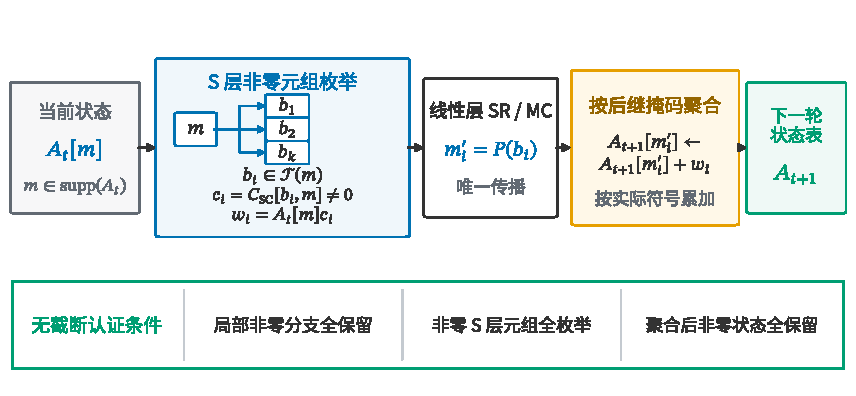
\includegraphics[width=14.3cm]{figures/fig1_certified_sparse_transition.pdf}
\caption{可认证稀疏路线壳求和的一轮状态转移. 对每个 $m\in\supp(A_t)$, 算法枚举非零 S 层元组, 经线性层唯一传播后, 按后继掩码进行带符号聚合. 局部非零分支、非零 S 层元组以及聚合后的非零状态全部保留时, 该轮满足无截断认证条件. }
\label{fig:transition}
\end{figure}

\section{正确性与数值表示}

\subsection{无截断认证下的路线壳完整性}

\begin{theorem}[无截断认证下的路线壳完整性]
固定轮数 $r$ 与输入掩码 $u$. 设一轮相关矩阵为 $\bm{R}=\bm{M}_{MC}\bm{M}_{SR}\bm{M}_{SC}$. 若算法 1 在 $r$ 轮传播中通过无截断认证, 则最终有限支撑状态表表示 $\bm{R}^{r}$ 的第 $u$ 列:
\begin{equation}
A_r=\bm{R}^{r}e_u.
\label{eq:main-theorem-vector}
\end{equation}
因此, 对任意输出掩码 $v\in\mathbb F_2^{32}$, 有
\begin{equation}
A_r[v]=\bm{M}(r)[v,u].
\label{eq:main-theorem-coordinate}
\end{equation}
\end{theorem}

\begin{proof}
初始化时 $A_0=e_u$. 以下用归纳法证明对所有 $t\ge 0$ 都有
\begin{equation}
A_t=\bm{R}^{t}e_u.
\label{eq:induction-invariant}
\end{equation}
当 $t=0$ 时, 结论由初始化直接成立.

假设式~\eqref{eq:induction-invariant} 对某个 $t$ 成立. 考虑第 $t+1$ 轮. 由于没有局部 S 盒分支截断和 S 层非零元组截断, 算法对每个当前掩码 $m$ 完整枚举所有满足 $\bm{M}_{SC}[b,m]\neq0$ 的 S 盒层输出掩码 $b$. 对每个这样的 $b$, 线性层由转置传播关系给出唯一后继掩码 $m'=P(b)$, 且线性层相关矩阵贡献为 1. 对落到同一 $m'$ 的贡献进行带符号聚合, 得到
\begin{equation}
A_{t+1}[m']=\sum_m A_t[m]\bm{R}[m',m].
\label{eq:induction-step}
\end{equation}
由归纳假设,
\begin{equation}
A_{t+1}[m']=\sum_m \bm{R}^{t}[m,u]\bm{R}[m',m]=\bm{R}^{t+1}[m',u].
\label{eq:induction-multiply}
\end{equation}
无状态剪枝保证所有非零后继均保留在有限支撑状态表中, 故式~\eqref{eq:induction-invariant} 对 $t+1$ 成立. 取 $t=r$, 并由 $\bm{M}(r)=\bm{R}^{r}$, 得到式~\eqref{eq:main-theorem-vector} 与式~\eqref{eq:main-theorem-coordinate}.
\end{proof}

负相关由带符号聚合自然处理. 零值过滤、零掩码排除和重复端点去重属于评测输出构造, 不影响上述代数等式.

\subsection{数值表示与误差边界}

定理 1 在实数域中的相关矩阵上成立. 局部 S 盒相关度来自 $2^{-4}$ 归一化 Walsh 和, 因此每条路线贡献及有限路线壳和均为二进有理数. 当前实现使用有限精度表示保存这些数值, 但不声称核心程序执行了通用大整数有理数运算. 为避免数值格式成为正确性缺口, 最终审计对每条记录重新运行方式二路线壳求和并比较复现值与记录值; 最终审计中 $VE$ 复现不匹配数为 0. 零值过滤和去重在输出构造阶段执行, 不参与定理 1 的证明.

\section{复杂度分析}

\subsection{方式一明文枚举基准}

对固定 $(r,u,v)$, 方式一在明文空间中计算
\begin{equation}
\bm{M}(r)[v,u]=2^{-32}\sum_{x\in\mathbb F_2^{32}}(-1)^{u^\top x\oplus v^\top HS(r)(x)}.
\label{eq:way1}
\end{equation}
该路径需要遍历 $2^{32}$ 个输入, 主复杂度为
\begin{equation}
T_{\mathrm{way1}}(r)=O(r\cdot 2^{32}).
\label{eq:way1-complexity}
\end{equation}

\subsection{固定输入掩码的路线空间代价}

\begin{proposition}[固定输入掩码的路线空间代价]
对固定 $(r,u)$, 设 $\mathcal A_t=\supp(A_t)$ 为第 $t$ 轮状态表的支撑集, $\tau_t(m)$ 为状态 $m$ 在第 $t$ 轮实际枚举的 S 层非零元组数. 若一次方式二运行没有状态剪枝, 则其路线空间展开规模为
\begin{equation}
T_{\mathrm{way2}}(r,u)=\sum_{t=0}^{r-1}\sum_{m\in\mathcal A_t}\tau_t(m).
\label{eq:way2-complexity}
\end{equation}
该量度量被枚举的非零路线前缀数量, 而不是完整 CPU 指令级运行时间.
\end{proposition}

审计中的“生成非零转移数”和“展开状态数”是实现级结构计数, 不包含全部哈希表操作、解析、输入输出、缓存效应或进程开销. 本文不以最终记录条数作为复杂度比较单位: 记录条数反映输出规模, 方式二的计算单位是固定 $(r,u)$ 的路线壳展开. 一次方式二运行可同时认证多个输出端点 $v$.

\subsection{复杂度审计结果}

\begin{table}[H]
\centering
\caption{按唯一 $(r,u)$ 汇总的复杂度审计结果}
\label{tab:complexity}
\zihao{-4}
\begin{tabularx}{0.93\textwidth}{L r}
\toprule
指标 & 数值 \\
\midrule
唯一 $(r,u)$ 数量 & 4760 \\
方式一基准 $2^{32}$ & 4294967296 \\
生成非零转移数达到或超过 $2^{32}$ 的 $(r,u)$ 数量 & 0 \\
展开状态数达到或超过 $2^{32}$ 的 $(r,u)$ 数量 & 0 \\
单个 $(r,u)$ 最大生成非零转移数 & 7578152 \\
最大生成非零转移数与 $2^{32}$ 的比值 & 0.00176443 \\
单个 $(r,u)$ 最大展开状态数 & 1001 \\
单个 $(r,u)$ 最大最终状态表规模 & 46453 \\
生成非零转移数中位数 & 68420 \\
生成非零转移数第 95 百分位 & 2648720 \\
展开状态数中位数 & 101 \\
展开状态数第 95 百分位 & 401 \\
\bottomrule
\end{tabularx}
\end{table}

最终结果集中没有任何唯一 $(r,u)$ 达到 $2^{32}$ 的明文枚举规模. 最大路线空间展开规模为 7578152, 仅为 $2^{32}$ 的 0.00176443.

\section{实验结果}

\subsection{最终有效记录与得分}

最终结果文件包含 138338 条有效记录. 按评测规则计算, 总分为 105843.622442471292742994. 按轮数统计见表~\ref{tab:score}.

\begin{table}[H]
\centering
\caption{最终有效记录与得分}
\label{tab:score}
\zihao{-4}
\begin{tabular}{rrrr}
\toprule
轮数 $r$ & 有效记录数 & 分数和 & 最高单条分数 \\
\midrule
1 & 288 & 288.000000 & 1 \\
2 & 90236 & 63893.609604 & 4 \\
3 & 47814 & 41662.012838471292742994 & 3 \\
\midrule
合计 & 138338 & 105843.622442471292742994 & 4 \\
\bottomrule
\end{tabular}
\end{table}

\subsection{输入活跃四比特字分布}

\begin{table}[H]
\centering
\caption{输入活跃四比特字分布}
\label{tab:active}
\zihao{-4}
\begin{tabular}{rrrr}
\toprule
轮数 $r$ & 活跃四比特字数 & 有效记录数 & 唯一输入掩码数 \\
\midrule
1 & 1 & 288 & 120 \\
2 & 1 & 3280 & 120 \\
2 & 2 & 72351 & 3477 \\
2 & 3 & 14605 & 947 \\
3 & 1 & 47430 & 90 \\
3 & 2 & 384 & 6 \\
\bottomrule
\end{tabular}
\end{table}

低活跃掩码区域是最终认证记录的主要来源. $r=2$ 的活跃二字记录贡献最大, 而线性近似表引导的 $r=3$ 活跃二字补充搜索增加了 384 条认证记录.

\subsection{全量审计}

\begin{table}[H]
\centering
\caption{最终结果集的全量审计摘要}
\label{tab:audit}
\zihao{-4}
\begin{tabularx}{0.80\textwidth}{L r}
\toprule
审计项 & 数值 \\
\midrule
输出记录数 & 138338 \\
审计记录数 & 138338 \\
有效记录数 & 138338 \\
无截断认证记录数 & 138338/138338 \\
$VE$ 复现不匹配记录数 & 0 \\
唯一 $(u,v)$ 数量 & 138338 \\
重复 $(u,v)$ 记录数 & 0 \\
$u=0$、$v=0$、$VT=0$、$VE=0$ 记录数 & 0 \\
\bottomrule
\end{tabularx}
\end{table}

全量审计验证了最终所有记录均满足定理 1 所需的代码级假设, 并且不存在无效掩码、零值或重复端点.

\subsection{方式一精确抽样复核}

方式一精确程序仅在最终结果生成完成后读取抽样端点, 独立计算参考值并进行一致性比较; 它不参与候选生成、排序、筛选或数值写入. 表~\ref{tab:spotcheck} 给出代表性样本, 完整摘要为 18 条查询、4 条 E06 活跃二字样本、不匹配数 0、最大绝对误差 0、最大相对误差 0.

\begin{table}[H]
\centering
\caption{方式一精确抽样复核的代表性样本}
\label{tab:spotcheck}
\zihao{5}
\begin{tabularx}{\textwidth}{L C{0.7cm} C{2.2cm} C{2.2cm} C{1.6cm} C{1.6cm} C{1.0cm}}
\toprule
类别 & $r$ & $u$ & $v$ & 路线壳值 & 方式一值 & 一致 \\
\midrule
一轮正值基线 & 1 & \code{0x00000001} & \code{0x80080000} & 0.5 & 0.5 & 是 \\
一轮负值基线 & 1 & \code{0x00000001} & \code{0x70070000} & -0.5 & -0.5 & 是 \\
二轮高分样本 & 2 & \code{0x00002000} & \code{0x08880000} & 1 & 1 & 是 \\
二轮活跃一字 & 2 & \code{0x00000001} & \code{0x0400e00e} & 0.1875 & 0.1875 & 是 \\
三轮活跃一字 & 3 & \code{0x00002000} & \code{0x04044440} & 0.125 & 0.125 & 是 \\
E06 活跃二字正值 & 3 & \code{0x00006060} & \code{0x04004004} & 0.125 & 0.125 & 是 \\
E06 活跃二字负值 & 3 & \code{0x00006060} & \code{0x08008008} & -0.125 & -0.125 & 是 \\
\bottomrule
\end{tabularx}
\end{table}

\subsection{Full exact-way2 与 Strategy-B Stage-A 证据}

最终收口阶段追加了 full exact-way2 双后端重算证据. 该证据对冻结结果中的 4760 个唯一 $(r,u)$ 列分别运行 \code{cpp\_int} 与 \code{int128\_checked} exact dyadic 后端, 并对 138338 个 frozen endpoint 进行精确整数比较. 结果为: 两个后端均完成 4760 列, 两个后端的 exact certificate 和 Parseval 检查均为 4760/4760; 138338 个 endpoint 全部为 \code{EXACT\_EQUAL}, \code{NOT\_EQUAL}、\code{PARSE\_ERROR} 和 \code{MISSING\_ENDPOINT} 均为 0; cross-backend mismatch counters 均为 0. 该证据闭合的是方式二数学与数值证据链, 产物位于 \code{artifacts/way2\_exact/full/}.

同时, Strategy-B Stage-A 对方式一 batch 工具链进行了小域正确性验证. Stage-A 覆盖 current、grouped-u 和 grouped-uv 三种实现、uniform / frozen-subset / synthetic-frozen-shaped 查询族、shard reducer 负例、GCC / Clang / UBSan / ASan / TSan 与 $-O0/-O3$ 一致性 gate. 结果为 A0、A1、A2 和 toolchain 均 PASS, numerator mismatch count 为 0, shard negative tests 为 12. 该阶段没有运行完整 $2^{32}$ 明文域, 没有运行全量 138338 查询 way-1, 也没有生成 Strategy-B final file; 因此它不构成 full way-1 $VT$ provenance.

\subsection{路线壳聚合机制示例}

一个最高单条分数样本为 $(r,u,v)=(2,\mathtt{0x00002000},\mathtt{0x08880000})$, 其路线壳求和值为 1. 该值不是由单条绝对值为 1 的路线产生, 而是由四条同号路线在共同端点处聚合得到, 如图~\ref{fig:hull-aggregation} 所示.

\begin{figure}[H]
\centering
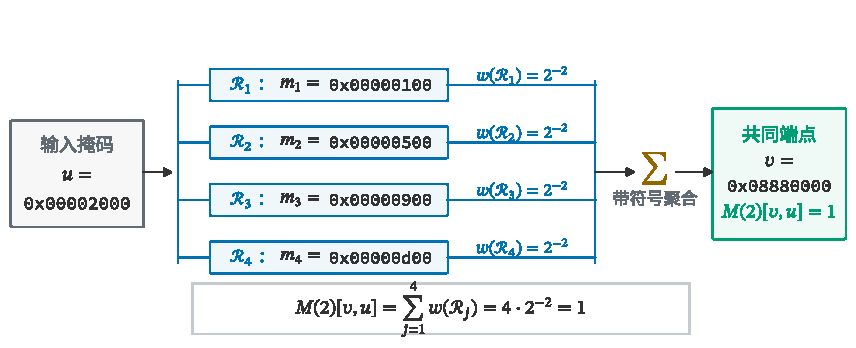
\includegraphics[width=14.2cm]{figures/fig2_linear_hull_aggregation.pdf}
\caption{四条同号线性路线在共同端点处的聚合. 四条路线经过不同的中间掩码到达同一端点, 每条路线贡献为 $2^{-2}$, 带符号聚合后得到 $\bm{M}(2)[v,u]=1$. 本例用于说明路线壳增强机制; 一般情形下, 路线贡献按照实际符号累加. }
\label{fig:hull-aggregation}
\end{figure}

该示例只用于解释端点聚合为何必要, 不承担最终结果正确性的证明责任; 最终正确性由定理 1 与全量无截断审计共同给出.

\section{线性近似表引导的补充搜索}

\subsection{数学动机}

S 盒层的局部线性近似表决定从一个活跃四比特字出发的非零分支数量和局部相关强度. 对于三轮低活跃掩码搜索, 输入活跃位置与局部掩码取值会显著影响路线空间展开规模. 因此, 补充搜索优先考虑活跃四比特字数为 2 且局部 LAT 分支结构较有利的输入模式. 该批次在复现材料中记为 E06.

\subsection{合入规则}

从 E06 候选来源中选取满足以下条件的记录: $r=3$; 活跃四比特字数为 2; 通过无截断认证; 单条分数为正; 输入掩码、输出掩码和数值均非零; 且不与既有 $(u,v)$ 冲突. 筛选仅使用方式二认证来源和审计信息, 不使用方式一精确输出进行候选排序、筛选或数值生成.

\subsection{结果}

E06 最终合入 384 条记录, 涉及 6 个唯一输入掩码. 所有合入记录均包含在最终全量审计中, 并满足与其余记录相同的无截断认证条件. 4 条 E06 样本进入方式一精确抽样复核, 不匹配数为 0.

\begin{table}[H]
\centering
\caption{E06 补充搜索摘要}
\label{tab:e06}
\zihao{-4}
\begin{tabular}{lr}
\toprule
项目 & 数值 \\
\midrule
合入的 $r=3$ 活跃二字记录数 & 384 \\
唯一活跃二字输入掩码数 & 6 \\
E06 精确抽样复核查询数 & 4 \\
E06 复核不匹配数 & 0 \\
\bottomrule
\end{tabular}
\end{table}

\section{声明、数学依据与复现材料依据}

正文仅保留最关键的声明-证据映射, 具体文件路径、命令和预期输出见附录 II 及仓库中的详细证据映射文件.

\begin{table}[H]
\centering
\caption{主要声明及其依据}
\label{tab:claims}
\zihao{-4}
\begin{tabularx}{\textwidth}{L L L}
\toprule
论文声明 & 数学依据 & 复现材料依据 \\
\midrule
认证运行满足 $A_r[v]=\bm{M}(r)[v,u]$ & 定理 1 & 全量无截断审计 \\
138338 条有效记录 & 评测有效性与评分规则 & 评分输出 \\
全部记录通过无截断认证 & 定义 1 与定理 1 假设 & 审计摘要 \\
唯一 $(r,u)=4760$ & 命题 2 的统计口径 & 复杂度摘要 \\
最大生成非零转移数 7578152 & 路线空间结构计数 & 复杂度摘要 \\
18 条精确抽样复核且不匹配数为 0 & 独立验证 & 精确复核摘要 \\
full exact-way2 双后端完成 4760 列 & exact dyadic 完整列重算与 endpoint 比较 & full exact-way2 摘要 \\
Strategy-B Stage-A 已 PASS & 小域 way-1 batch 工具链验证 & Stage-A 摘要 \\
\bottomrule
\end{tabularx}
\end{table}

\section{消融观察与方法解释}

本文不将消融实验作为最终正确性证据. 消融实验的作用是解释候选发现阶段的设计选择, 而非证明最终记录正确; 最终正确性由定理 1 与全量无截断审计支撑.

若仅保留单条路线, 就无法解释多个中等贡献路线在同一端点处同向叠加的现象. 按端点进行带符号聚合更符合线性壳定义. 搜索规模的作用主要体现在能否获得无截断认证: 一旦发生局部分支、S 层元组或聚合状态剪枝, 对应输出只能作为候选, 不能作为最终认证记录.

\section{评测输出字段来源}

最终结果文件包含评测格式要求的两个数字字段 $VT$ 与 $VE$. 对无截断认证记录, 方式二完整路线壳求和得到的数值等于目标相关矩阵坐标. 因此, 当前冻结结果文件中的两个数字字段具有相同数值. 该数值来自方式二的可认证完整路线壳求和, 不是复制方式一明文枚举输出. 方式一全量 $VT$ provenance 尚未闭合; 当前方式一证据包括 18 条独立抽样复核和 Strategy-B Stage-A 工具链验证.

\section{局限性与未来工作}

本文方法面向低活跃掩码区域, 并依赖路线空间稀疏性. 对于高活跃掩码, S 层元组数和中间状态数可能迅速增长, 使无截断认证更难获得. 随着轮数增加, 线性层扩散也会放大中间状态表规模.

本文不声称完成全部掩码空间的最优搜索, 也不声称对所有轮数均能高效给出完整线性壳. 本文的结论仅针对最终结果集中通过无截断认证的记录: 这些记录的方式二路线壳求和在数学上等于对应矩阵坐标.

未来可研究双向线性壳拼接、较高轮数候选搜索、轮函数结构对称性以及精确二进有理数累加. 这些方向不是本文最终结果的一部分, 也未参与当前结果文件构造.

\section{结论}

本文提出 SPN 型置换相关矩阵坐标的可认证稀疏路线壳求和方法. 该方法利用 S 盒层克罗内克积结构和线性层转置传播关系, 在掩码路线空间中枚举非零路线前缀, 并按后继掩码进行带符号聚合. 无截断认证把候选搜索与最终数值生成严格区分开来; 定理 1 证明认证运行满足 $A_r=\bm{R}^{r}e_u$, 因而输出等于完整线性壳和 $\bm{M}(r)[v,u]$.

在评测实例上, 最终结果集包含 138338 条有效记录, 总分为 \seqsplit{105843.622442471292742994}. 全部记录均通过无截断认证, 方式二审计复现不匹配数为 0, 不存在零掩码、零值和重复端点; full exact-way2 双后端重算完成 4760 列并确认 138338 个 endpoint 全部 \code{EXACT\_EQUAL}; 18 条方式一独立抽样复核与方式二认证值完全一致; Strategy-B Stage-A 验证了 bounded way-1 batch 工具链, 但尚未启动 full $2^{32}$ 或全量 138338 查询 way-1. 因此, 当前结果由数学模型、正确性定理、按唯一 $(r,u)$ 的复杂度分析、全量审计、full exact-way2 证据和独立抽样复核共同支撑, 同时不声称 full way-1 $VT$ provenance 已闭合.

% 参考文献
\section*{\heiti\zihao{4} 参考文献}
\addcontentsline{toc}{section}{参考文献}
\noindent{\songti\zihao{4}
[1] 全国高校密码数学挑战赛组委会. 第十一届(2026年)全国高校密码数学挑战赛赛题三:矩阵连乘元素的逼近[Z]. 2026.\par
[2] 全国高校密码数学挑战赛组委会. 赛题附件程序 \texttt{computecor.cpp}. Linear Correlation Calculator[CP]. 2026.\par
[3] MATSUI M. Linear cryptanalysis method for DES cipher[C]//Advances in Cryptology-EUROCRYPT'93. Berlin:Springer,1994:386-397.\par
[4] NYBERG K. Linear approximation of block ciphers[C]//Advances in Cryptology-EUROCRYPT'94. Berlin:Springer,1995:439-444.\par
[5] BEYNE T. A geometric approach to linear cryptanalysis[C]//Advances in Cryptology-ASIACRYPT 2021,Part I. Cham:Springer,2021:36-66.\par}

% 附录
\clearpage
\section*{附录 I\quad 评测实例与输出格式}
\addcontentsline{toc}{section}{附录 I 评测实例与输出格式}

评测实例给定一个 32 比特替换-置换网络结构, 一轮为 $F=MC\circ SR\circ SC$. 相关矩阵连乘定义为 $\bm{M}(r)=\bm{M}_{3r-1}\bm{M}_{3r-2}\cdots\bm{M}_0$. 每条评测记录包含 $(r,u,v,VT,VE)$. 对本文最终无截断认证记录, 方式二完整路线壳求和给出 $\bm{M}(r)[v,u]$, 因此两个数字字段具有相同数值. 单条有效记录得分为
\[
\log_2\!\left(2^{2r}|VE|\right).
\]
最终得分为所有有效记录得分之和.

\section*{附录 II\quad 复现材料与独立复核}
\addcontentsline{toc}{section}{附录 II 复现材料与独立复核}

复现流程包括编译与测试、结果文件重建、评分、全量审计、复杂度摘要、full exact-way2 证据检查、Strategy-B Stage-A 证据检查和方式一抽样复核. 主要命令如下:

\begin{verbatim}
make clean && make -j
make test
python3 experiments/build_submit_from_sources.py \
  --out /tmp/submit_rebuilt.txt
cmp submit.txt /tmp/submit_rebuilt.txt
./score --dedup uv --positive-only submit.txt
python3 experiments/check_submission.py \
  --submit submit.txt
\end{verbatim}

预期评分输出为:
\begin{verbatim}
valid_count = 138338
total_score = 105843.622442471292742994
\end{verbatim}

当前证据状态边界为:
\begin{verbatim}
FULL_EXACT_WAY2_CLOSED
Strategy-B Stage-A = STAGE_A_PASS
stage_b_authorized=false
full_2_32_run_started=false
full_138338_way1_started=false
new_way1_run_started=false
strategy_b_final_file_generated=false
submit_txt_modified=false
vt_provenance_closed=false
\end{verbatim}

结果生成链与独立复核链的边界如图~\ref{fig:provenance} 所示. 最终结果由方式二可认证稀疏路线壳求和生成; 方式一只在结果生成后读取抽样端点与方式二结果, 独立计算参考值并进行一致性比较.

\begin{figure}[H]
\centering
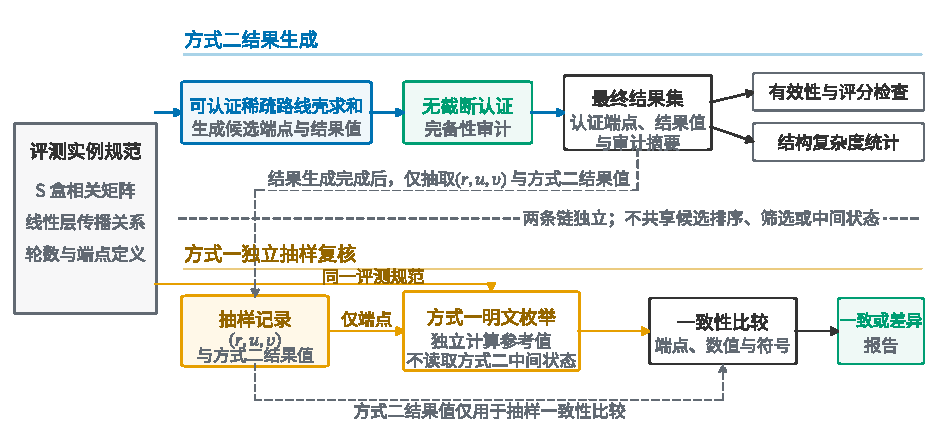
\includegraphics[width=15.7cm]{figures/figA1_generation_verification_boundary.pdf}
\caption{方式二结果生成链与方式一独立抽样复核链. 最终结果由方式二的可认证稀疏路线壳求和产生; 方式一仅在结果生成完成后读取抽样端点及其方式二数值, 独立计算参考值并进行一致性比较. }
\label{fig:provenance}
\end{figure}

\noindent{\heiti 复现材料索引: }
\begin{verbatim}
方式二候选来源
       |
       v
最终结果文件
       +-- 评分摘要
       +-- 无截断审计
       +-- 复杂度摘要
       +-- 精确抽样复核摘要
\end{verbatim}

详细声明-证据映射、输入文件、输出文件、验证命令和预期结果记录在仓库的 \code{docs/CLAIMS\_AND\_EVIDENCE.md} 中.

\end{document}
